%====================================================================================
\section{El comando \texttt{regress}}
%====================================================================================

\begin{frame}[fragile]{Sintaxis del comando de regresi�n}
	La sintaxis del comando de regresi�n de Stata describe las reglas del lenguaje de programaci�n Stata para la regresi�n.
			$$\cdot\enskip \textup{\texttt{regress} \enskip \textcolor{blue}{\textit{\texttt{depvar}}} \enskip [\textcolor{blue}{\textit{\texttt{indpvars}}}] \enskip [\textcolor{blue}{\textit{\texttt{if}}}] \enskip [\textcolor{blue}{\textit{\texttt{in}}}] \enskip [\textcolor{blue}{,\enskip \textit{\texttt{options}}}]}$$
	algunos ejemplos
\begin{lstlisting}[language=Stata, numbers=none]
use "http://www.ats.ucla.edu/stat/stata/dae/crime", clear
regress crime poverty single
\end{lstlisting}
\end{frame}
%---------------------------------------------------
\begin{frame}[fragile]{Sintaxis del comando de regresi�n}
\begin{lstlisting}[language=Stata, numbers=none]
use "http://www.ats.ucla.edu/stat/stata/dae/crime", clear
regress crime poverty single
\end{lstlisting}
	\begin{figure}
		\centering
		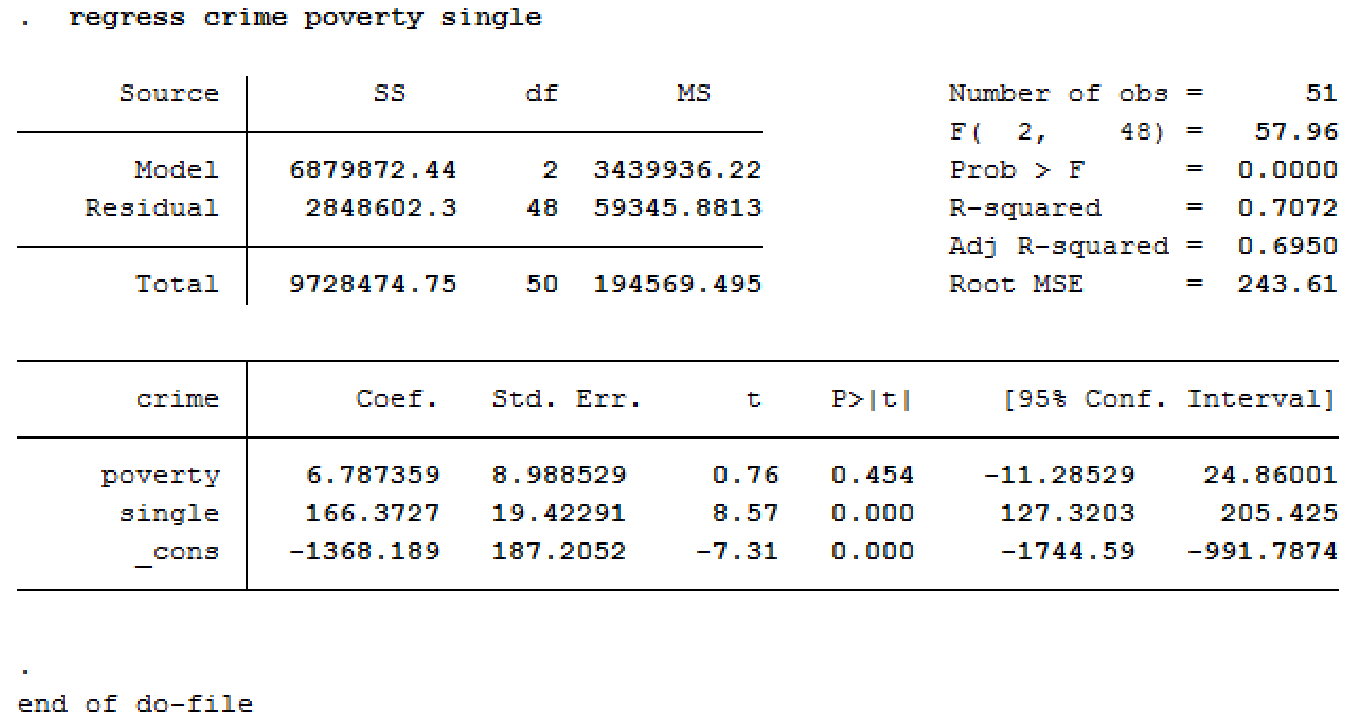
\includegraphics[width = 0.75\linewidth]{fig/regression.png}
	\end{figure}
\end{frame}
